\documentclass[a4paper,12pt]{article} % добавить leqno в [] для нумерации слева
\usepackage[a4paper,top=1.3cm,bottom=2cm,left=1.5cm,right=1.5cm,marginparwidth=0.75cm]{geometry}
%%% Работа с русским языком
\usepackage{cmap}					% поиск в PDF
\usepackage[warn]{mathtext} 		% русские буквы в фомулах
\usepackage[T2A]{fontenc}			% кодировка
\usepackage[utf8]{inputenc}			% кодировка исходного текста
\usepackage[english,russian]{babel}	% локализация и переносы
\usepackage{physics}
\usepackage{multirow}
\usepackage{bm}
\usepackage{longtable}
\usepackage{xcolor}
%%% Нормальное размещение таблиц (писать [H] в окружении таблицы)
\usepackage{float}
\restylefloat{table}


\documentclass[a4paper,12pt]{article}
\usepackage[utf8]{inputenc}
\usepackage[russian]{babel}
\usepackage{amsmath}
\usepackage{amssymb}
\usepackage{graphicx}
\usepackage{geometry}
\usepackage{booktabs}
\usepackage{caption}
\usepackage{enumitem}
\usepackage{siunitx}

\geometry{left=2cm,right=1.5cm,top=2cm,bottom=2cm}
\setlist[enumerate]{label=\arabic*., leftmargin=*}


\usepackage{graphicx}

\usepackage{wrapfig}
\usepackage{tabularx}

\usepackage{hyperref}
\usepackage[rgb]{xcolor}
\hypersetup{
	colorlinks=true,urlcolor=blue
}
\usepackage{pgfplots}
\pgfplotsset{compat=1.9}
%%% Дополнительная работа с математикой
\usepackage{amsmath,amsfonts,amssymb,amsthm,mathtools} % AMS
\usepackage{icomma} % "Умная" запятая: $0,2$ --- число, $0, 2$ --- перечисление

%% Номера формул
%\mathtoolsset{showonlyrefs=true} % Показывать номера только у тех формул, на которые есть \eqref{} в тексте,

%% Шрифты
\usepackage{euscript}	 % Шрифт Евклид
\usepackage{mathrsfs} % Красивый матшрифт

\title{Архитектура вычислительных систем. Домашнее задание №1. Вариант №3.}
\author{Комиссаров Данил Андреевич}
\date{March 2025}

\begin{document}

\maketitle
\section{Полный отчет}
Третий вариант задания. Полный сумматор (Full Adder) двух 3-битных входов.\\
Пожалуй будет сначала интересно рассмотреть некоторые аспекты построения и анализа схемы.
\subsection{Подсчет транзисторов для базовых элементов}
Доступные элементы для составления схемы:
\begin{enumerate}
    \item NOT Gate
    \item AND Gate
    \item NAND Gate
    \item OR Gate
    \item NOR GATE
    \item XOR GATE
    \item Probe
    \item Pin
    \item Соединительные провода
\end{enumerate}
Сразу же подсчитаем количество транзисторов в каждом логическом элементе:
\begin{itemize}
\item Известно, что оптимальная реализация NOT Gate использует 2 транзистора.
\begin{figure}[H]
    \centering
    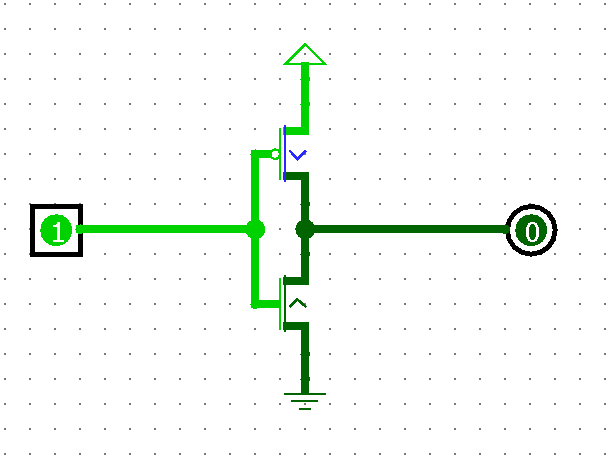
\includegraphics[width=0.5\linewidth]{Gates/NOT.png}
\end{figure}
Можно, конечно же, реализовать инвертор и на одном транзисторе при помощи одного транзистора и подтягивающего резистора.
\begin{figure}[H]
    \centering
    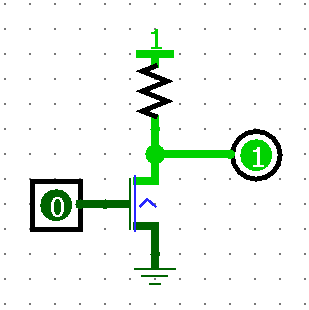
\includegraphics[width=0.25\linewidth]{Contrexamples/NOT Gate.png}
\end{figure}
Но это не соответствует КМОП логике из-за протекающего тока через подтягивающий резистор в стабильном состоянии. Жаль. Идем дальше.\\
\item Известно, что оптимальная реализация NAND Gate использует 4 транзистора.
\begin{figure}[H]
    \centering
    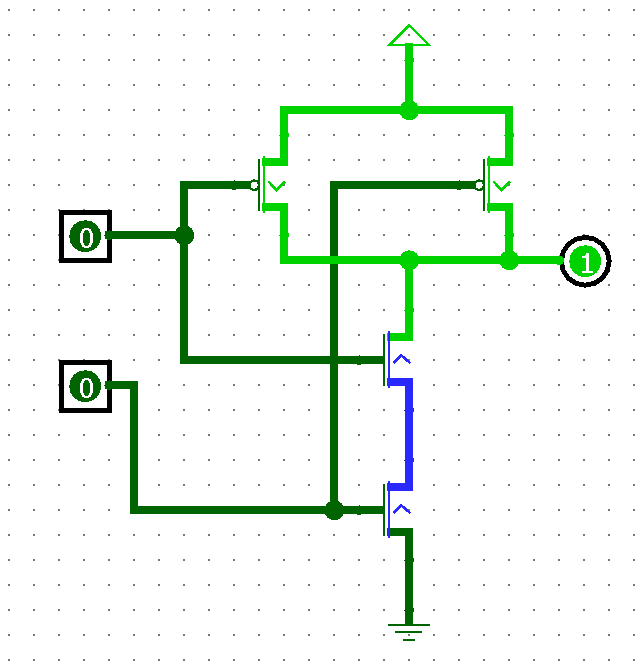
\includegraphics[width=0.5\linewidth]{Gates/NAND.png}
\end{figure}
Элемент NAND известен также как "Штрих Шеффера". Интересен он тем, что образует функционально-полный логический базис для пространства булевых функций от двух переменных, так как удовлетворяет теореме Поста о полной системе функций. В электронике это означает, что для реализации любой логической схемы достаточно одного типового элемента. С другой стороны, такой подход увеличивает громоздкость и тем самым снижает их надёжность. В этом задании я поставлю себе задачу реализовать конечное решение с использованием наименьшего количества транзисторов.\\
\item Элемент AND Gate реализуется точно так же, как и предыдущий, с точностью до замены всех типов транзисторов на противоположные.
\begin{figure}[H]
    \centering
    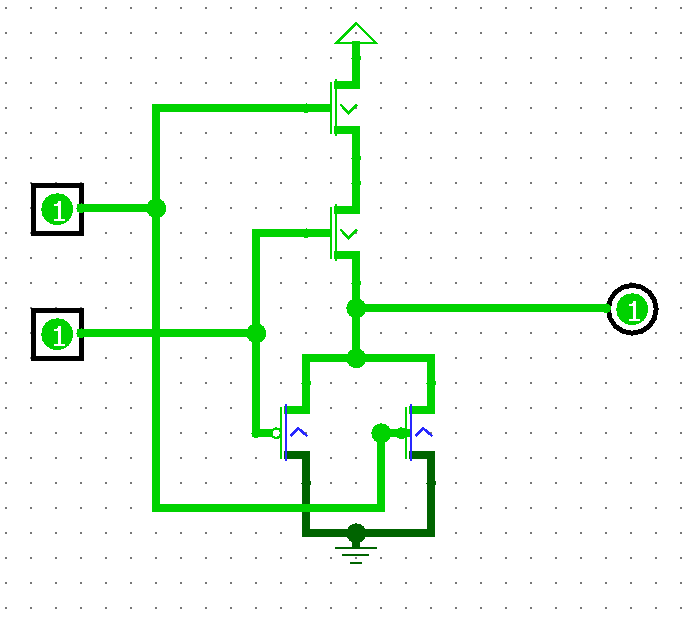
\includegraphics[width=0.5\linewidth]{Gates/AND.png}
\end{figure}
Впрочем, это верно и для любых других пар противоположных логических элементов.\\
\item Известно, что оптимальная реализация OR Gate использует 4 транзистора.
\begin{figure}[H]
    \centering
    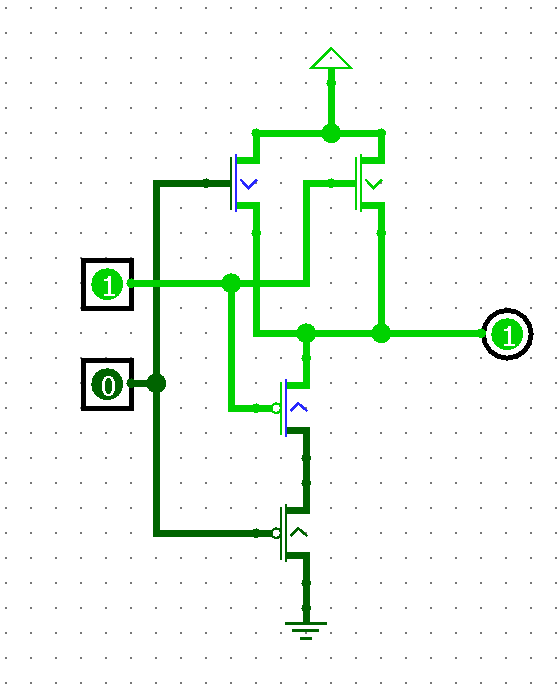
\includegraphics[width=0.5\linewidth]{Gates/OR Gate.png}
\end{figure}
\item Аналогично NOR Gate.
\begin{figure}[H]
    \centering
    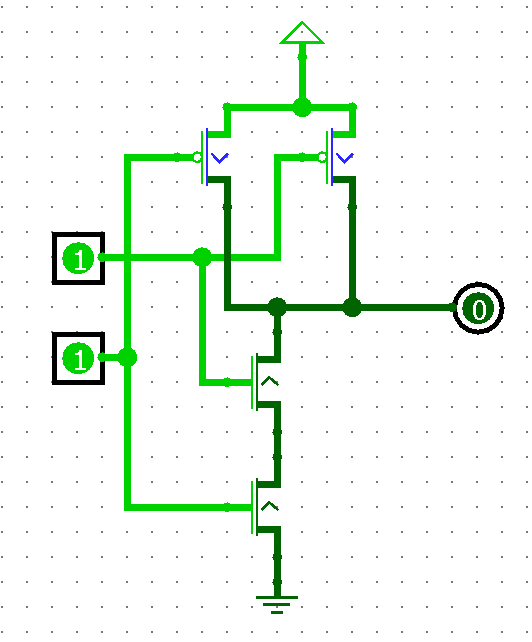
\includegraphics[width=0.5\linewidth]{Gates/NOR Gate.png}
\end{figure}
\item Теперь добрались до самого сложного: XOR Gate. \\

У нас нет элемента исключающего ИЛИ (XOR). Нужно реализовать его на базе других логических элементов. Как это сделать? Какое минимальное количество элементов придется использовать?\\
Для начала вспомним таблицу истинности для XOR.

\begin{table}[H] % Используем H для фиксирования таблицы
    \centering
    \begin{tabular}{|c|c|c|}
    \hline
    A & B & A XOR B \\
    \hline
    0 & 0 & 0 \\
    0 & 1 & 1 \\
    1 & 0 & 1 \\
    1 & 1 & 0 \\
    \hline
    \end{tabular}
\end{table}

Что делать? Нужно избавиться от самого оператора XOR. Для этого можем расписать функцию по таблице истинности двумя способами. Существуют такие вещи как \textbf{СКНФ}(совершенная конъюнктивная нормальная форма) и \textbf{СДНФ}(совершенная дизъюнктивная нормальная форма).
Впрочем эти вещи эквивалентны друг другу, т.к. равны одной и той же функции. Поэтому не принципиально, каким методом пользоваться. Можно даже показать это:
\[
a \text{ xor } b = ( \overline{a} \land b ) \lor ( a \land \overline{b} ) = \overline{a} \cdot b + a \cdot \overline{b} =
\]
\[
= ( \overline{a} \cdot b + a ) \cdot ( a \cdot b + \overline{b} ) = 
\]
\[
= (1 \cdot (b + a)) \cdot ((\overline{a} + \overline{a}) \cdot (b + a) \cdot (b + \overline{b})) =
\]
\[
= (a + b) \cdot (a + b) = (a + b) \cdot (\overline{a} \cdot b)
\]
Итак, есть две формы:
\[
a \text{ xor } b = \overline{a} \cdot b + a \cdot \overline{b}
\]
\[
a \text{ xor } b = (a + b) \cdot (\overline{a} \cdot b)
\]
Обратите внимание, чаще всего везде используется первая формула. Но проблема в том, что для её построения на логических элементах нам нужно 5 логических элементов:
\begin{figure}[H]
    \centering
    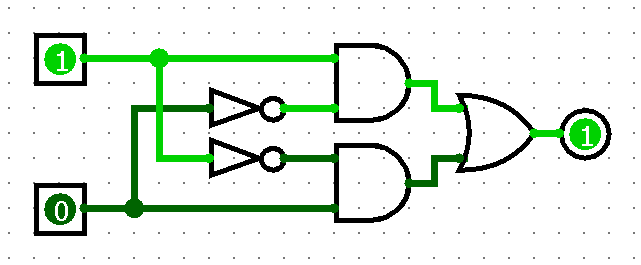
\includegraphics[width=0.5\linewidth]{Contrexamples/XOR1.png}
\end{figure}
Если же мы возьмем вторую формулу, то нам удастся реализовать XOR, используя только три элемента: NAND, OR, AND.
\begin{figure}[H]
    \centering
    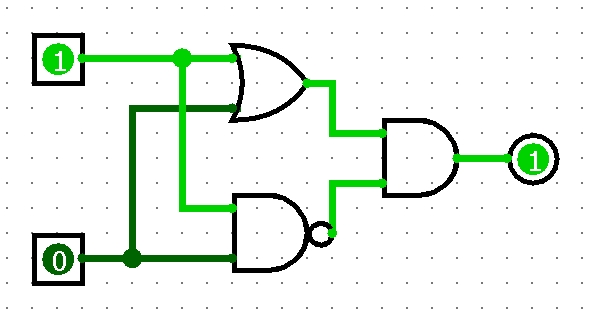
\includegraphics[width=0.5\linewidth]{Contrexamples/XOR2.png}
\end{figure}
А что если собрать только на NAND?
\[
a = \overline{a} + a = a \cdot a = (a \text{ nand } a)
\]
\[
a + b = a \cdot b = (\overline{a} + \overline{a}) \cdot (\overline{b} + \overline{b}) = (a \text{ nand } a) \text{ nand } (b \text{ nand } b)
\]
\[
a \cdot b = a \cdot b = a \cdot b \cdot a \cdot b = (a \text{ nand } b) \text{ nand } (a \text{ nand } b)
\]
Выражаем XOR через NAND:
\[
a \text{ xor } b = (a + b) \cdot \overline{(a \cdot b)} = 
\]
\[
= \overline{\overline{(a \cdot a)} \cdot \overline{(b \cdot b)}} \cdot \overline{(a \cdot b)} =  \overline{\overline{\overline{(a \cdot a)} \cdot \overline{(b \cdot b)}} \cdot \overline{(a \cdot b)}} \cdot  \overline{\overline{\overline{(a \cdot a)} \cdot \overline{(b \cdot b)}} \cdot \overline{(a \cdot b)}}
\]
\begin{figure}[H]
    \centering
    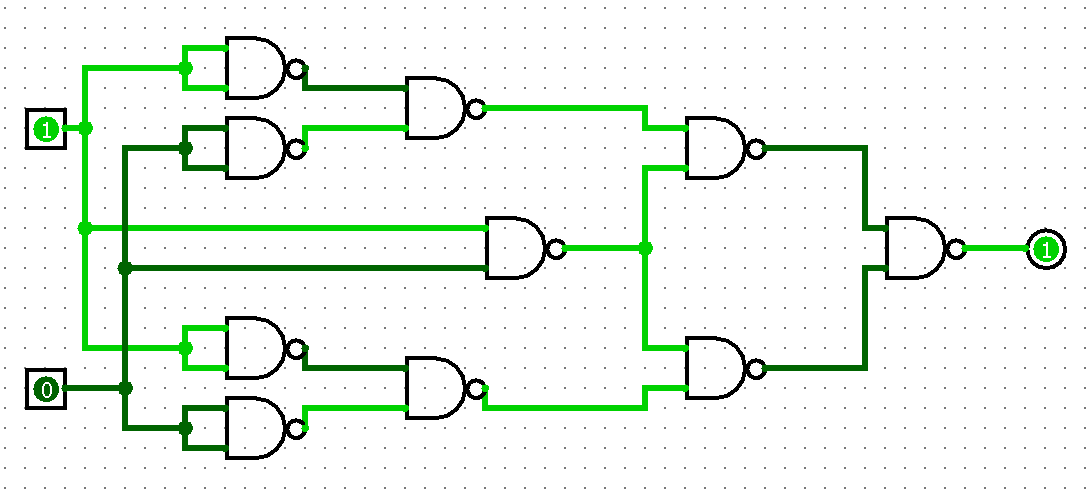
\includegraphics[width=1\linewidth]{Contrexamples/XOR3.png}
\end{figure}
Получилось очевидно громоздко, и даже встроенный анализ Logisim дает результат намного лучше.
\begin{figure}[H]
    \centering
    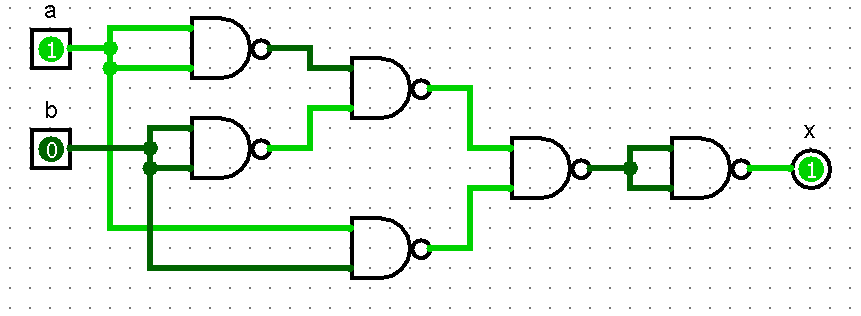
\includegraphics[width=0.75\linewidth]{Contrexamples/XOR4.png}
\end{figure}
Впрочем, очевидно и то, как можно еще сильнее сократить формулу.
\[
a \text{ xor } b = (a + b) \cdot (\overline{a \cdot b}) = a \cdot (\overline{(a \cdot b)}) + b \cdot (\overline{(a \cdot b)}) =
\]
\[
= a \cdot (\overline{(a \cdot b)}) \cdot b \cdot (\overline{(a \cdot b)})
\]
\begin{figure}[H]
    \centering
    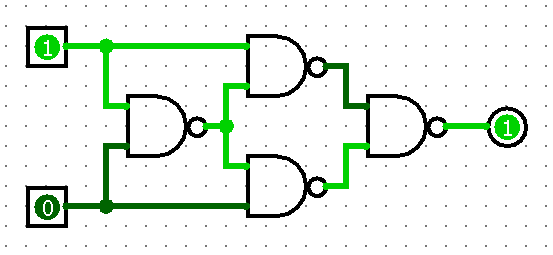
\includegraphics[width=0.5\linewidth]{Contrexamples/XOR5.png}
\end{figure}
Теперь это можно и расписать в транзисторах.
\begin{figure}[H]
    \centering
    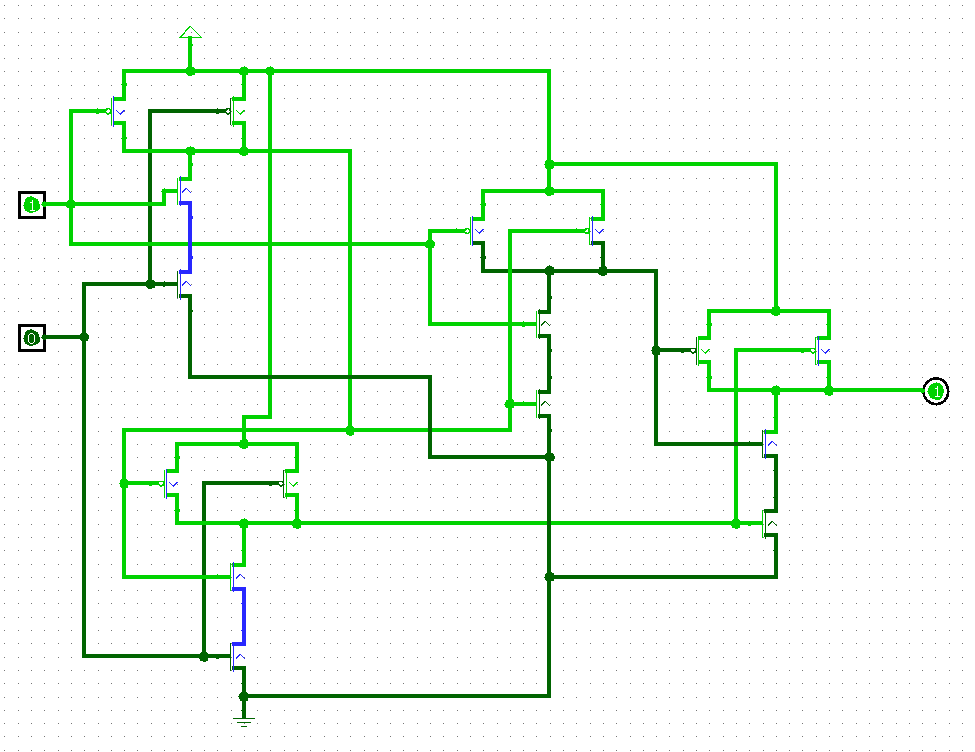
\includegraphics[width=1\linewidth]{Contrexamples/XOR6.png}
\end{figure}
Раскрытие элементов позволяет снова увидеть некоторые паттерны в схеме и сократить схему до конечного:
\begin{figure}[H]
    \centering
    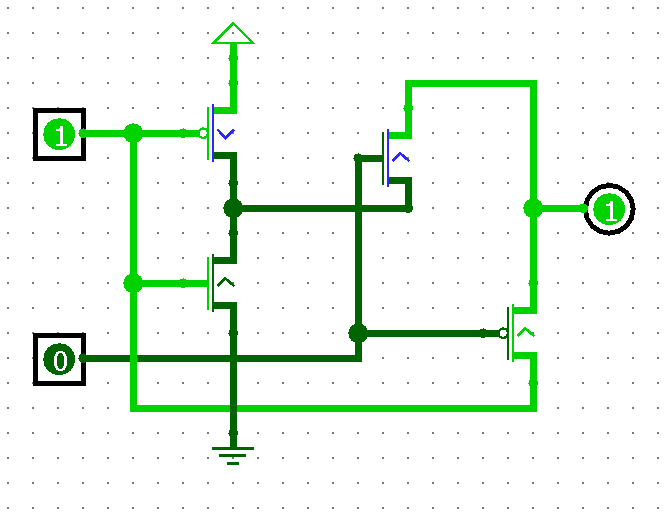
\includegraphics[width=0.5\linewidth]{Gates/XOR Gate.png}
\end{figure}
Дальнейшее упрощение не представляется возможным.\\
\item Элемент NXOR Gate аналогичен.
\begin{figure}[H]
    \centering
    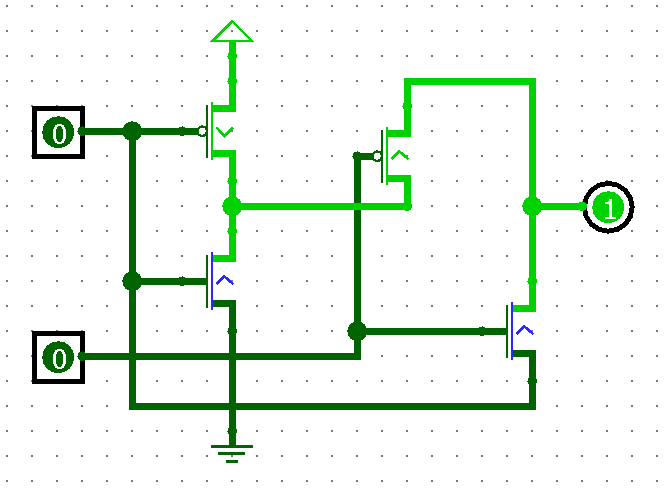
\includegraphics[width=0.5\linewidth]{Gates/NXOR Gate.png}
\end{figure}
\end{itemize}
\begin{table}[H]
    \centering
    \begin{tabular}{@{}ll@{}}
        \toprule
        Логический элемент & Кол-во т-ров \\ \midrule
        NOT Gate          & 2                       \\
        AND Gate          & 4                       \\
        NAND Gate         & 4                       \\
        OR Gate           & 4                       \\
        NOR Gate          & 4                       \\
        XOR Gate          & 4                       \\ \bottomrule
    \end{tabular}
\end{table}
Подсчитали наконец-то. Теперь можно и начинать составлять схему сумматора.
\subsection{Составление схемы сумматора}
Опираться придется на материалы из лекции.
Сначала собирается полусумматор:
\begin{figure}[H]
    \centering
    \begin{minipage}{0.35\linewidth} % 45% ширины для первой картинки
        \centering
        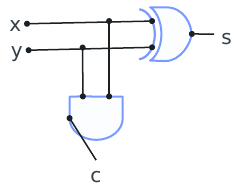
\includegraphics[width=\linewidth]{Progress/semi-adder.png}
    \end{minipage}%
    \hspace{0.05\linewidth} % Пробел между картинками
    \begin{minipage}{0.45\linewidth} % 45% ширины для второй картинки
        \centering
        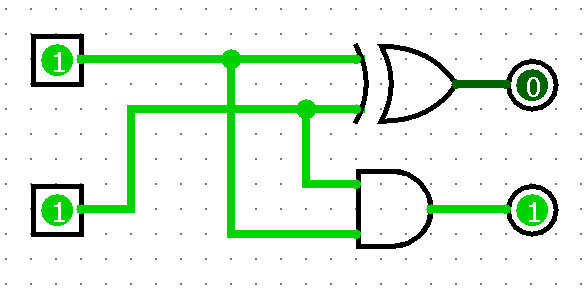
\includegraphics[width=\linewidth]{Progress/semi-adder1.png}
    \end{minipage}
\end{figure}
Тривиально.\\
Далее собираем из них полные сумматоры.
\begin{figure}[H]
    \centering
    \begin{minipage}{0.35\linewidth} % 45% ширины для первой картинки
        \centering
        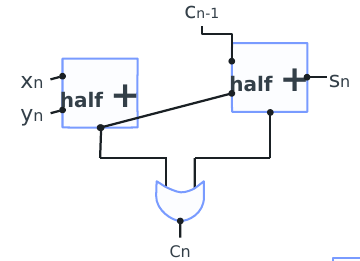
\includegraphics[width=\linewidth]{Progress/adder.png}
    \end{minipage}%
    \hspace{0.05\linewidth} % Пробел между картинками
    \begin{minipage}{0.50\linewidth} % 45% ширины для второй картинки
        \centering
        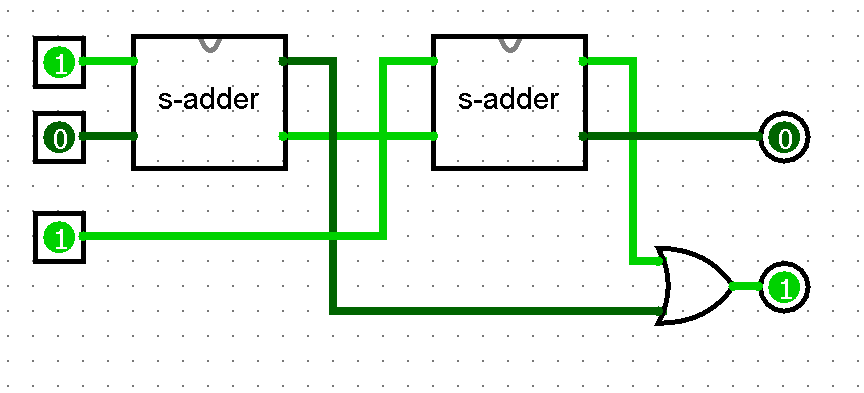
\includegraphics[width=\linewidth]{Progress/adder1.png}
    \end{minipage}
\end{figure}
А теперь просто каскадируем их.
\begin{figure}[H]
    \centering
    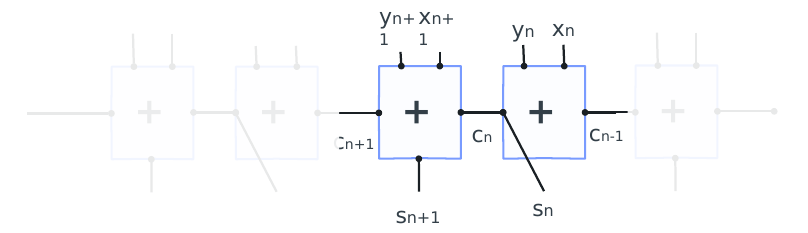
\includegraphics[width=1\linewidth]{Progress/3bit-adder.png}
\end{figure}
\begin{figure}[H]
    \centering
    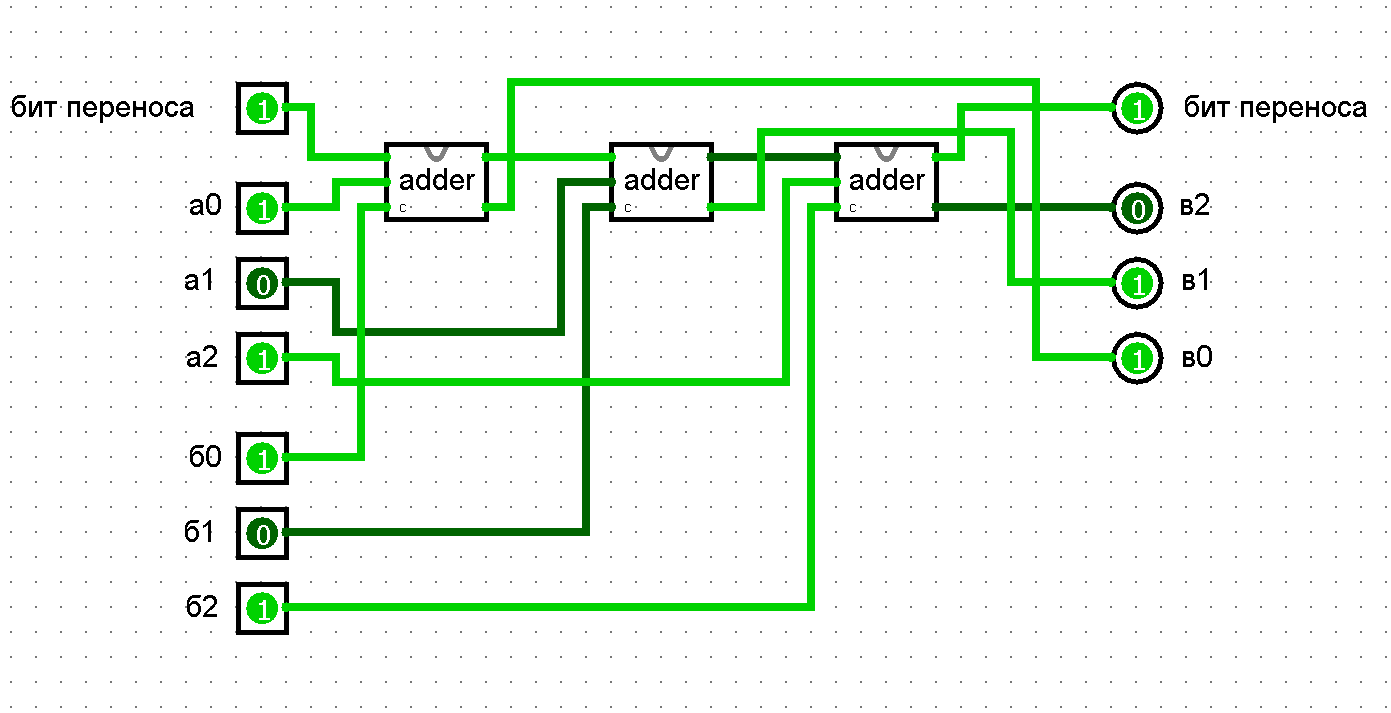
\includegraphics[width=1\linewidth]{Progress/3bit-adder1.png}
\end{figure}
Итого:
\begin{figure}[H]
    \centering
    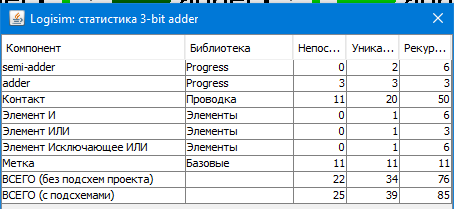
\includegraphics[width=0.75\linewidth]{Progress/3bit-adder2.png}
\end{figure}
\begin{table}[H]
    \centering
    \begin{tabular}{@{}llr@{}}
        \toprule
        \textbf{Компонент}                    & \textbf{Рекур.} & \textbf{Кол-во т-ров.} \\ \midrule
        Элемент И                            & 6               & 24                    \\
        Элемент ИЛИ                          & 3               & 12                    \\
        Элемент Исключающее ИЛИ              & 6               & 24                    \\ \midrule
        \textbf{Итого}                       &                 & \textbf{60}          \\ 
        \bottomrule
    \end{tabular}
\end{table}
Здорово. Но помимо этого можно и доверить построение схемы самому Logisim.
Воспользуемся встроенным сумматором (приходится расписывать однобитными элементами, т.к. к сожалению анализ схемы с многобитными элементами недоступен).
\begin{figure}[H]
    \centering
    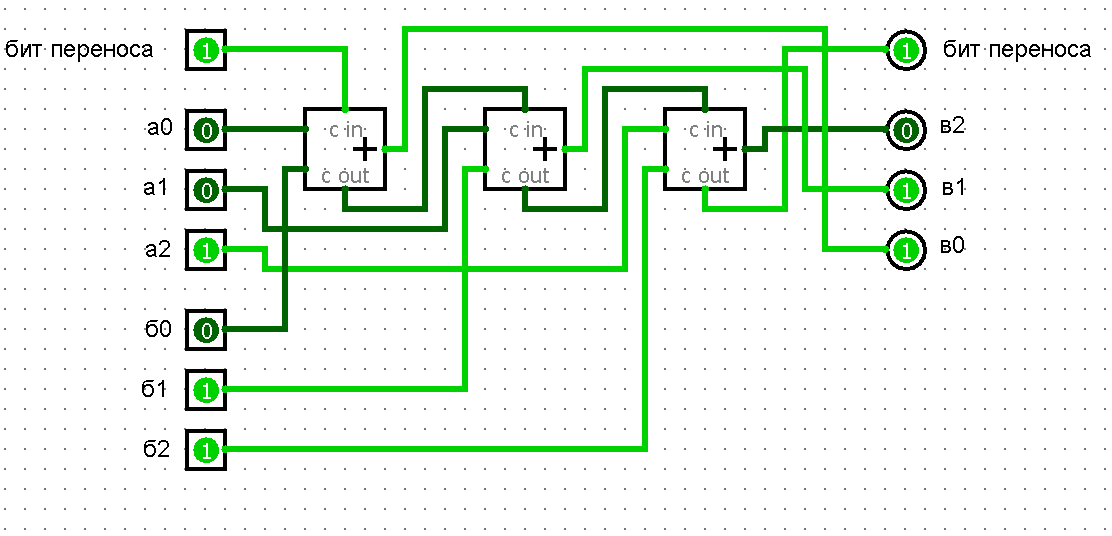
\includegraphics[width=0.75\linewidth]{Progress/computer adder.png}
\end{figure}
А теперь компьютер раскроет схему.
\begin{figure}[H]
    \centering
    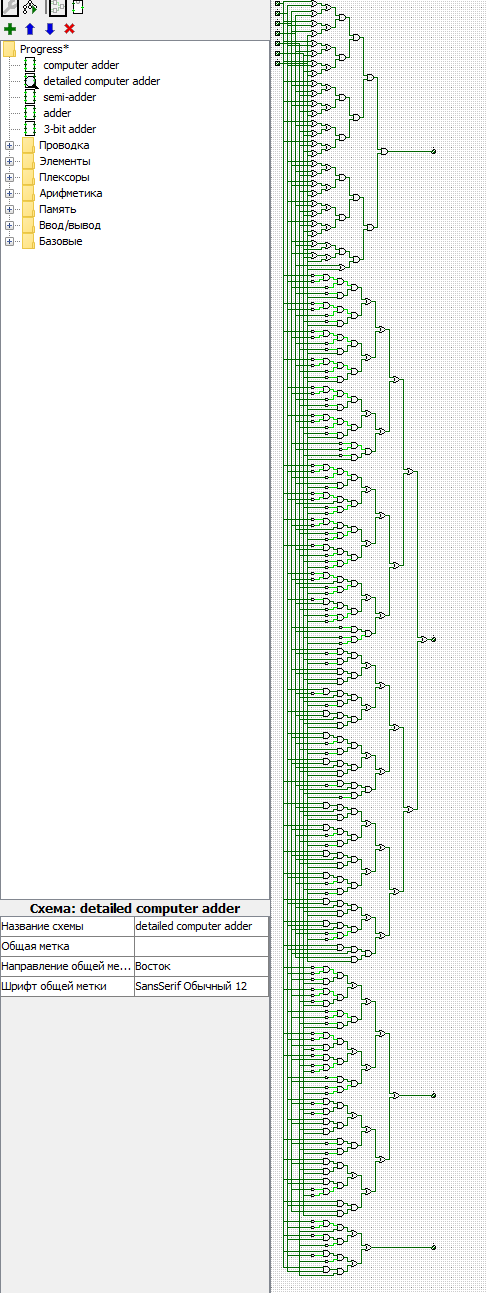
\includegraphics[width=0.5\linewidth]{Progress/detailed computer adder.png}
\end{figure}
Получилось довольно громоздко.
\begin{figure}[H]
    \centering
    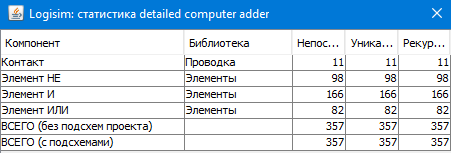
\includegraphics[width=0.5\linewidth]{Progress/detailed computer adder1.png}
\end{figure}
И статистика говорит о том же. Предлагаю тогда остановиться на предыдущем результате. \\
Тогда разобьем схему на элементы, разрешенные в задании, чтобы посчитать критический путь (предполагается, что каждый элемент из списка занимает одинаковое время). 
\begin{figure}[H]
    \centering
    \includegraphics[width=1\linewidth]{crit way.png}
\end{figure}
Итого 9t (хотя интересно, что в предыдущем варианте, предоставленный компьютером, критическое время составляло всего 7t).
Помимо прочего, можно уточнить, что это за время t такое. Если вернуться к подсекции "Подсчет транзисторов для базовых элементов", то можно заметить, что каждый из базовых элементов имеет критическое время в 1 транзистор (это только в том случае, если принять, что не требуется ожидания для сигнала при прохождении через открытый транзистор, т.е. путь коллектор-эмиттер не занимает время), т.е. для получения стабильного сигнала на выходе требуется подождать одно характерное время работы транзистора, поэтому и правда есть обоснование в том, чтобы уравнять характерные времена базовых элементов.\\
Когда все аспекты рассмотрены, можно занять написание "формального отчета".
\section{Формальный отчет}
\begin{enumerate}
    \item Выполнил: Комиссаров Данил Андреевич.
    \item Студент группы Б01-304.
    \item Выполненная схема - Полный сумматор (Full Adder) двух 3-битных входов.
    \item Контакты: komissarov.da@phystech.edu
    \item Полный сумматор — логическая схема, которая производит сложение двух трехбитных чисел и одного однобитного числа, обозначаемых A(а0 - младший бит, а1 - средний бит, а2 - старший бит), Б(б0 - младший бит, б1 - средний бит, б2 - старший бит) и входной бит переноса. На выход подаются трехбитное число В(в0 - младший бит, в1 - средний бит, в2 - старший бит) и выходной бит переноса., где В — это сумма по модулю 8 (а в общем случае $2^n$), а выходной бит переноса - это флаг, который говорит о переполнении выхода.
    \item 
    \begin{figure}[H]
        \centering
        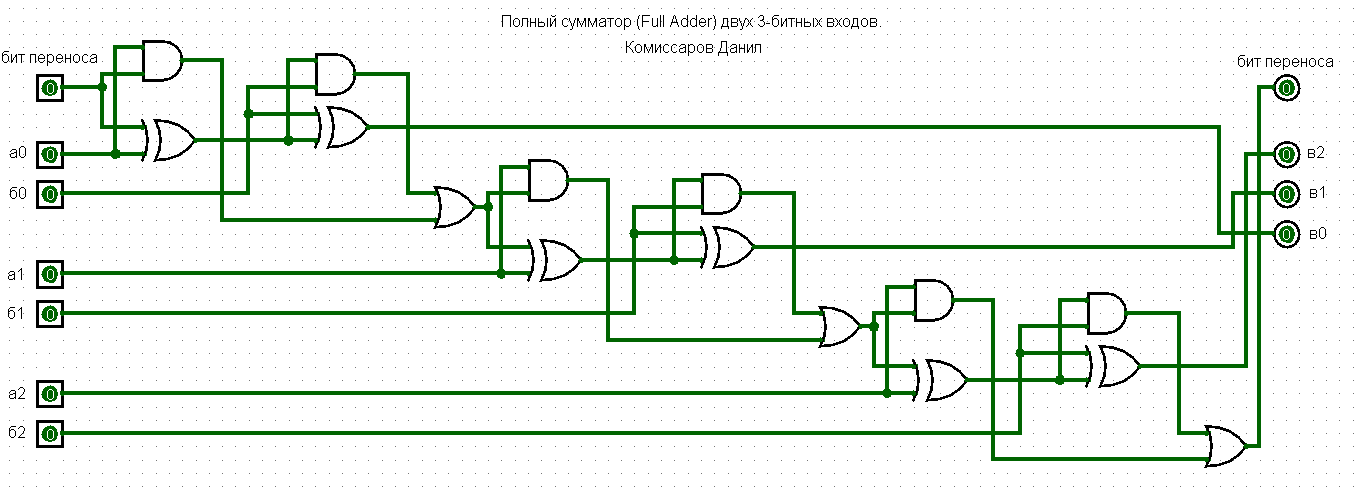
\includegraphics[width=1\linewidth]{Formal/Photo1.png}
    \end{figure}
    \begin{figure}[H]
        \centering
        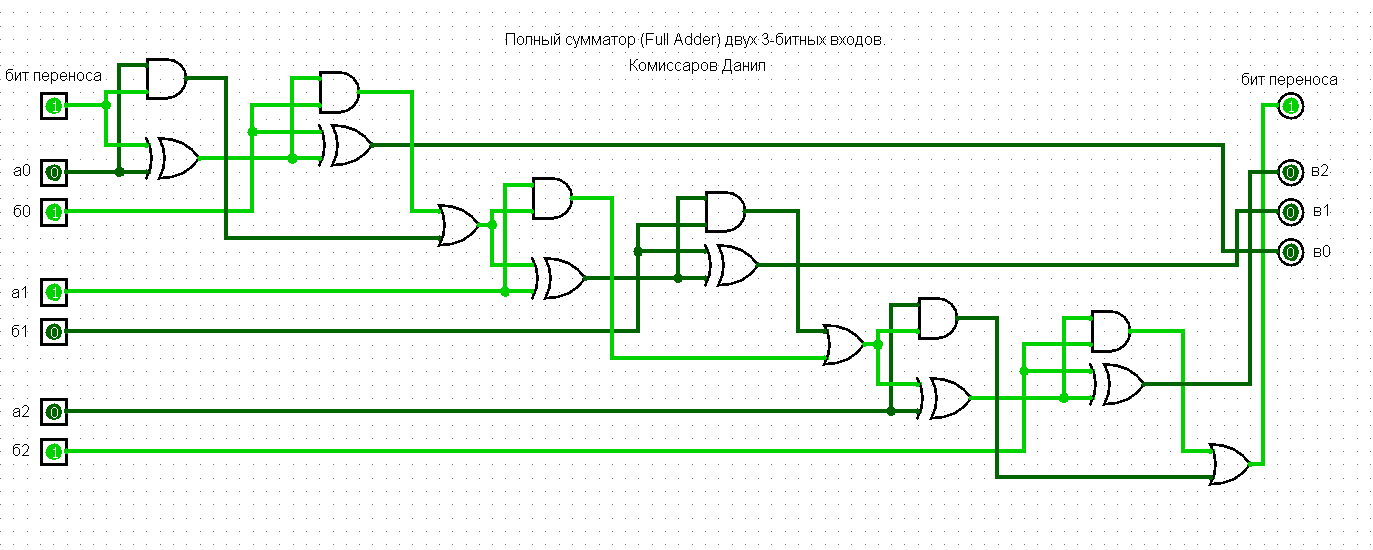
\includegraphics[width=1\linewidth]{Formal/Photo2.png}
    \end{figure}
    \begin{figure}[H]
        \centering
        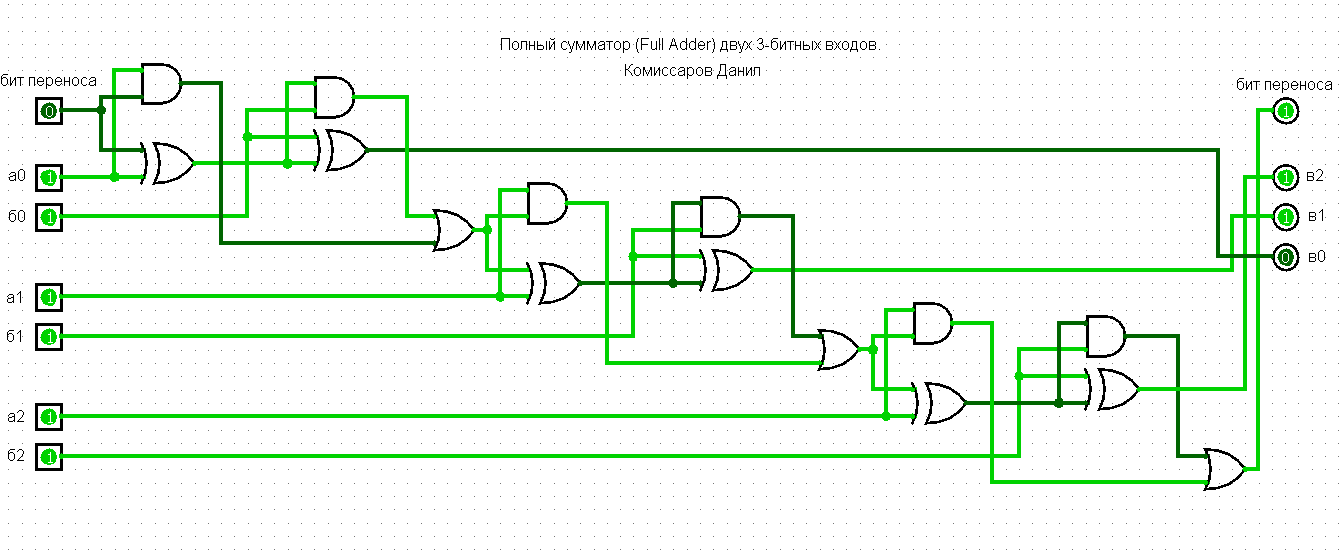
\includegraphics[width=1\linewidth]{Formal/Photo3.png}
    \end{figure}
    \begin{figure}[H]
        \centering
        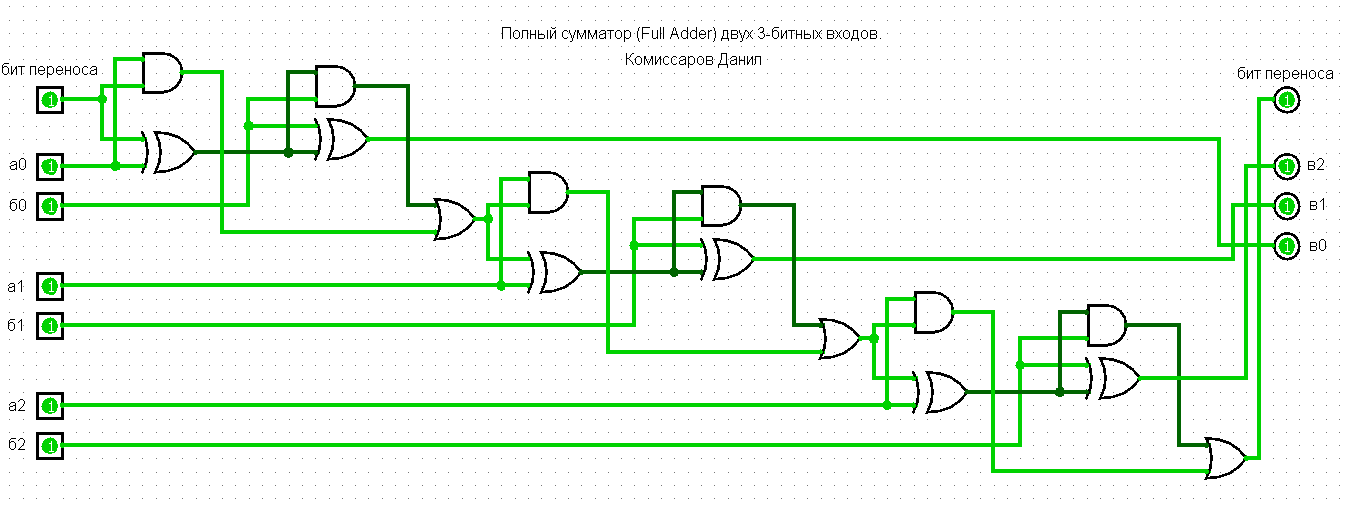
\includegraphics[width=1\linewidth]{Formal/Photo4.png}
    \end{figure}
    \item 
    \begin{figure}[H]
        \centering
        \includegraphics[width=1\linewidth]{Formal/Crit way.png}
    \end{figure}
    Критическое время составляет 9t
    \item 
    Схема состоит из 60-ти полевых транзисторов.
\end{enumerate}
На этом пожалуй можно и закончить. Наверное я уделил слишком много внимания несущественным аспектам, в то время, когда некоторые фундаментальные принципы были упущены, но это было интересно. 
\end{document}
